\documentclass[12pt,french]{report}
\usepackage[T1]{fontenc}
\usepackage[utf8]{inputenc}
\usepackage{lmodern}
\usepackage[a4paper,right=2.5cm,left=2.5cm,bottom=2.5cm, inner=2.5cm,outer=2.5cm]{geometry}
\usepackage{babel}
\usepackage{blindtext}
\usepackage{multirow}
\usepackage{placeins}
\usepackage{array}
\usepackage{float}
\usepackage{tikz}
\usetikzlibrary{shadows}
\usepackage{xcolor,colortbl}

\usepackage{graphicx}
\usepackage{fancyhdr}

\usepackage{hyperref}
\hypersetup{
	colorlinks,
	citecolor=black,
	filecolor=black,
	linkcolor=black,
	urlcolor=black
}

\graphicspath{{images}}

\pagestyle{fancy}

\newcommand{\thedate}{\today}


\begin{document}
	\begin{titlepage}
		\begin{center}
			\large Algérienne Démocratique et Populaire\\
			
			\large Ministère de l’Enseignement Supérieur et de la Recherche Scientifique
			
			\large Université Constantine 2 – AbdelHamid Mehri\\
			
			\vspace{0.01\textheight}
			
\includegraphics[width=0.2\textheight]{logo.jpg}\\
			
			Faculté des Nouvelles Technologies de l’Information et de la Communication\\
			Département des Technologies des Logiciels et Systèmes d’Information\\
			
			\vspace{0.025\textheight}
			\par\noindent\rule{10cm}{3pt}\\
			\vspace{0.05\textheight}
			
			\large{Projet de fin d’études pour l’obtention du diplôme de Licence en Informatique}\\
			
			\vspace{0.025\textheight}
			Option: Génie Logiciel\\
			
			\vspace{0.025\textheight}			
			\textbf{\large{Thème}}
			
			\vspace{0.025\textheight}			
			
\begin{tikzpicture}
				\node [copy shadow={fill=black,shadow xshift=0.5ex,shadow yshift=-0.5ex},
				fill=white,draw=black,thick,font=\bfseries] {\textbf{\LARGE Application pour embaucher des artisans}};
			\end{tikzpicture}
		\end{center}
	
		\vspace{0.05\textheight}

		\begin{tabular}{l l}
			\Large Dirigé par & \Large Réalisé par\\
			\multirow{1}{24em}{\large{- Dr. LAKHDARA Zakaria}} & \large{- Boudaakkar Nazih}\\
			& \large{- Bekakria Abir}\\
			& \large{- Fermas Manar}\\
		\end{tabular}
		\vspace{4.3em}
		
		\centering
		- Session Juin 2021 -
	\end{titlepage}
\tableofcontents
\listoffigures
\listoftables

\pagebreak
\section{Introduction général}

Le monde connaît un développement très rapide au niveau de technologie informatique. La gestion informatisée de la plupart des systèmes qui simplifie la majorité de nos taches quotidienne, mais malheureusement y a certain certains domaines non touchés\\
``Connais-tu un bon plombier?''
\hfill
ou
\hfill
``Si quelqu’un cherche un maçon, contacte-moi''.

\noindent Ce sont des phrases trop communes dans notre société, un artisan qui cherche un client pour gagner un peux d'argent ou une personne ayant un problème de soudure ou problème de plomberie et elle cherche un artisan qualifié pour le résoudre.\\

Durant notre vie quotidienne, on a souvent besoins de certains services de bricolage (remplacer une prise ou placer un chauffage central) mais malheureusement le temps passé à la recherche d’un bon artisans n’est pas court et parfois en se fait trompé par un artisan qui fais seulement un demis travail ou bien aucun travail.
\subsection*{Solution}
Une plateforme dans laquelle un utilisateur (client) peut trouver et contacter un artisan spécialisé dans le domaine requis sans énormes efforts et recherches qui durent longtemps.
Dans cette plateforme, un visiteur sera présenté par une liste des artisans disponible avec touts détailles nécessaires comprenant le prix, l’adresse, le numéro de téléphone, le nom et le prénom, ensuite le visiteur peut choisir de contacter un artisans- directement en utilisant le numéro de téléphone ou bien s’inscrire pour lui contacter dans la plateforme et discuter les détailles du projet.

Ce travail sera divisé en trois chapitres:
\begin{enumerate}
	\item Le premier chapitre sera dédié pour l’analyse des besoins, le cahier des charges, l'identification des acteurs et enfin la liste des besoins fonctionnels et non-fonctionnels.
	\item Le deuxième chapitre contient la conception du projet qui consiste des diagrammes de séquences, diagrammes d’activés, diagramme de classe final et en fin le schéma de la base de données.
	\item Le troisième chapitre contient des détailles sur l’implémentation et la réalisation de l’application ainsi qu’une petite discussion sur les technologies utiliséesLe premier chapitre sera dédié pour l’analyse des besoins, le cahier des charges, l’identification des acteurs et enfin la liste des besoins fonctionnels et non-fonctionnels
\end{enumerate}



\chapter{Analyse des besoins}
Dans l'analyse des besoins on prend compte les nécessités de l'application et du client en analysant les fonctionnalités demandées en établissant un cahier des charges

\section{Cahier des charges}
Un cahier des charges est la première étape dans chaque projet, il
sert à formaliser les besoins et à les expliquer aux différents acteurs pour s’assurer que tout le monde soit d’accord.

\subsection{Identification des acteurs et leurs besoins}
Un acteur, autrement dit utilisateur, est une personne qui engage avec le système, soit d'une façon direct ou indirect.

\begin{enumerate}
	\item \textcolor{red}{Administrateur}: Il est le garant du développement, déroulement  et de l'évolution du site.\\
	Il peut:
	\begin{itemize}
		\item Gérer les comptes des utilisateurs (Ajouter, Modifier, Bloquer, Supprimer).
		\item Gérer les appels d’offres et les soumissions (Ajouter, Modifier, Supprimer).
		\item Gérer les réclamations et les signalements.
	\end{itemize}

	\item \textcolor{red}{Visiteur}: Qui entre sur le site pour la première fois avant d'ouvrir un compte.\\
	Il peut:
	\begin{itemize}
		\item Consulter site  via une application web ou mobile.
		\item S'inscrire dans le site pour devenir un client.
		\item Consulter la liste et les profils des artisans.
	\end{itemize}

	\item \textcolor{red}{Client}: Visiteur ayant un compte.\\
	Il peut:
	\begin{itemize}
		\item Gérer son profil.
		\item Consulter la liste et les profils des artisans.
		\item Poster un appel d’offre.
		\item Gérer ses appels d’offres (Modifier ou Supprimer).
		\item Gérer les soumissions des artisans pour un appel d’offre.
		\item Demander le service d’un artisan.
		\item Évaluer le service d’un artisan.
		\item Signaler un artisan et soumettre une réclamation.
	\end{itemize}

	\item \textcolor{red}{Artisan}: Qui possède un métier, que ce soit maçon, couvreur, plombier, tapissier, chauffagiste, coiffeur, fleuriste, tailleur$\dots$\\
	Il peut:
	\begin{itemize}
		\item Gérer son profile.
		\item Consulter des appels d’offres.
		\item Soumettre des appels d’offres.
		\item Gérer soumissions (Modifier ou Supprimer).
		\item Évaluer un client.
		\item Signaler un client.
	\end{itemize}
\end{enumerate}

\subsection{Besoins non-fonctionnels}
Les besoins non-fonctionnels sont des nécessités non-visible pour l'utilisateur mais sont nécessaires pour avoir une douce expérience dans l'application.\\
\begin{itemize}
\item Le système doit être disponible tout le temps.
\item Le système doit être facile a utiliser.
\item Temps de réponse très court.
\item Les mots de passe sont stockés de manière sécurisée.
\item Le système suffisamment intuitif pour faciliter l’opération au client.
\end{itemize}


\pagebreak
\section{Spécification des besoins}
La spécification des besoins et le premier document produit dans le chapitre d'analyse, elle consiste a décrire les fonctionnalités et leurs contraintes d'une façon simple et lisible a fin de pouvoir les communiquer facilement

\subsection{Diagramme Cas D'utilisation}
Un diagramme de cas d'utilisation nous permet de visualiser les besoins / fonctionnalités de l'application d'une façon abstraite.

\begin{figure}[h!]
\centering
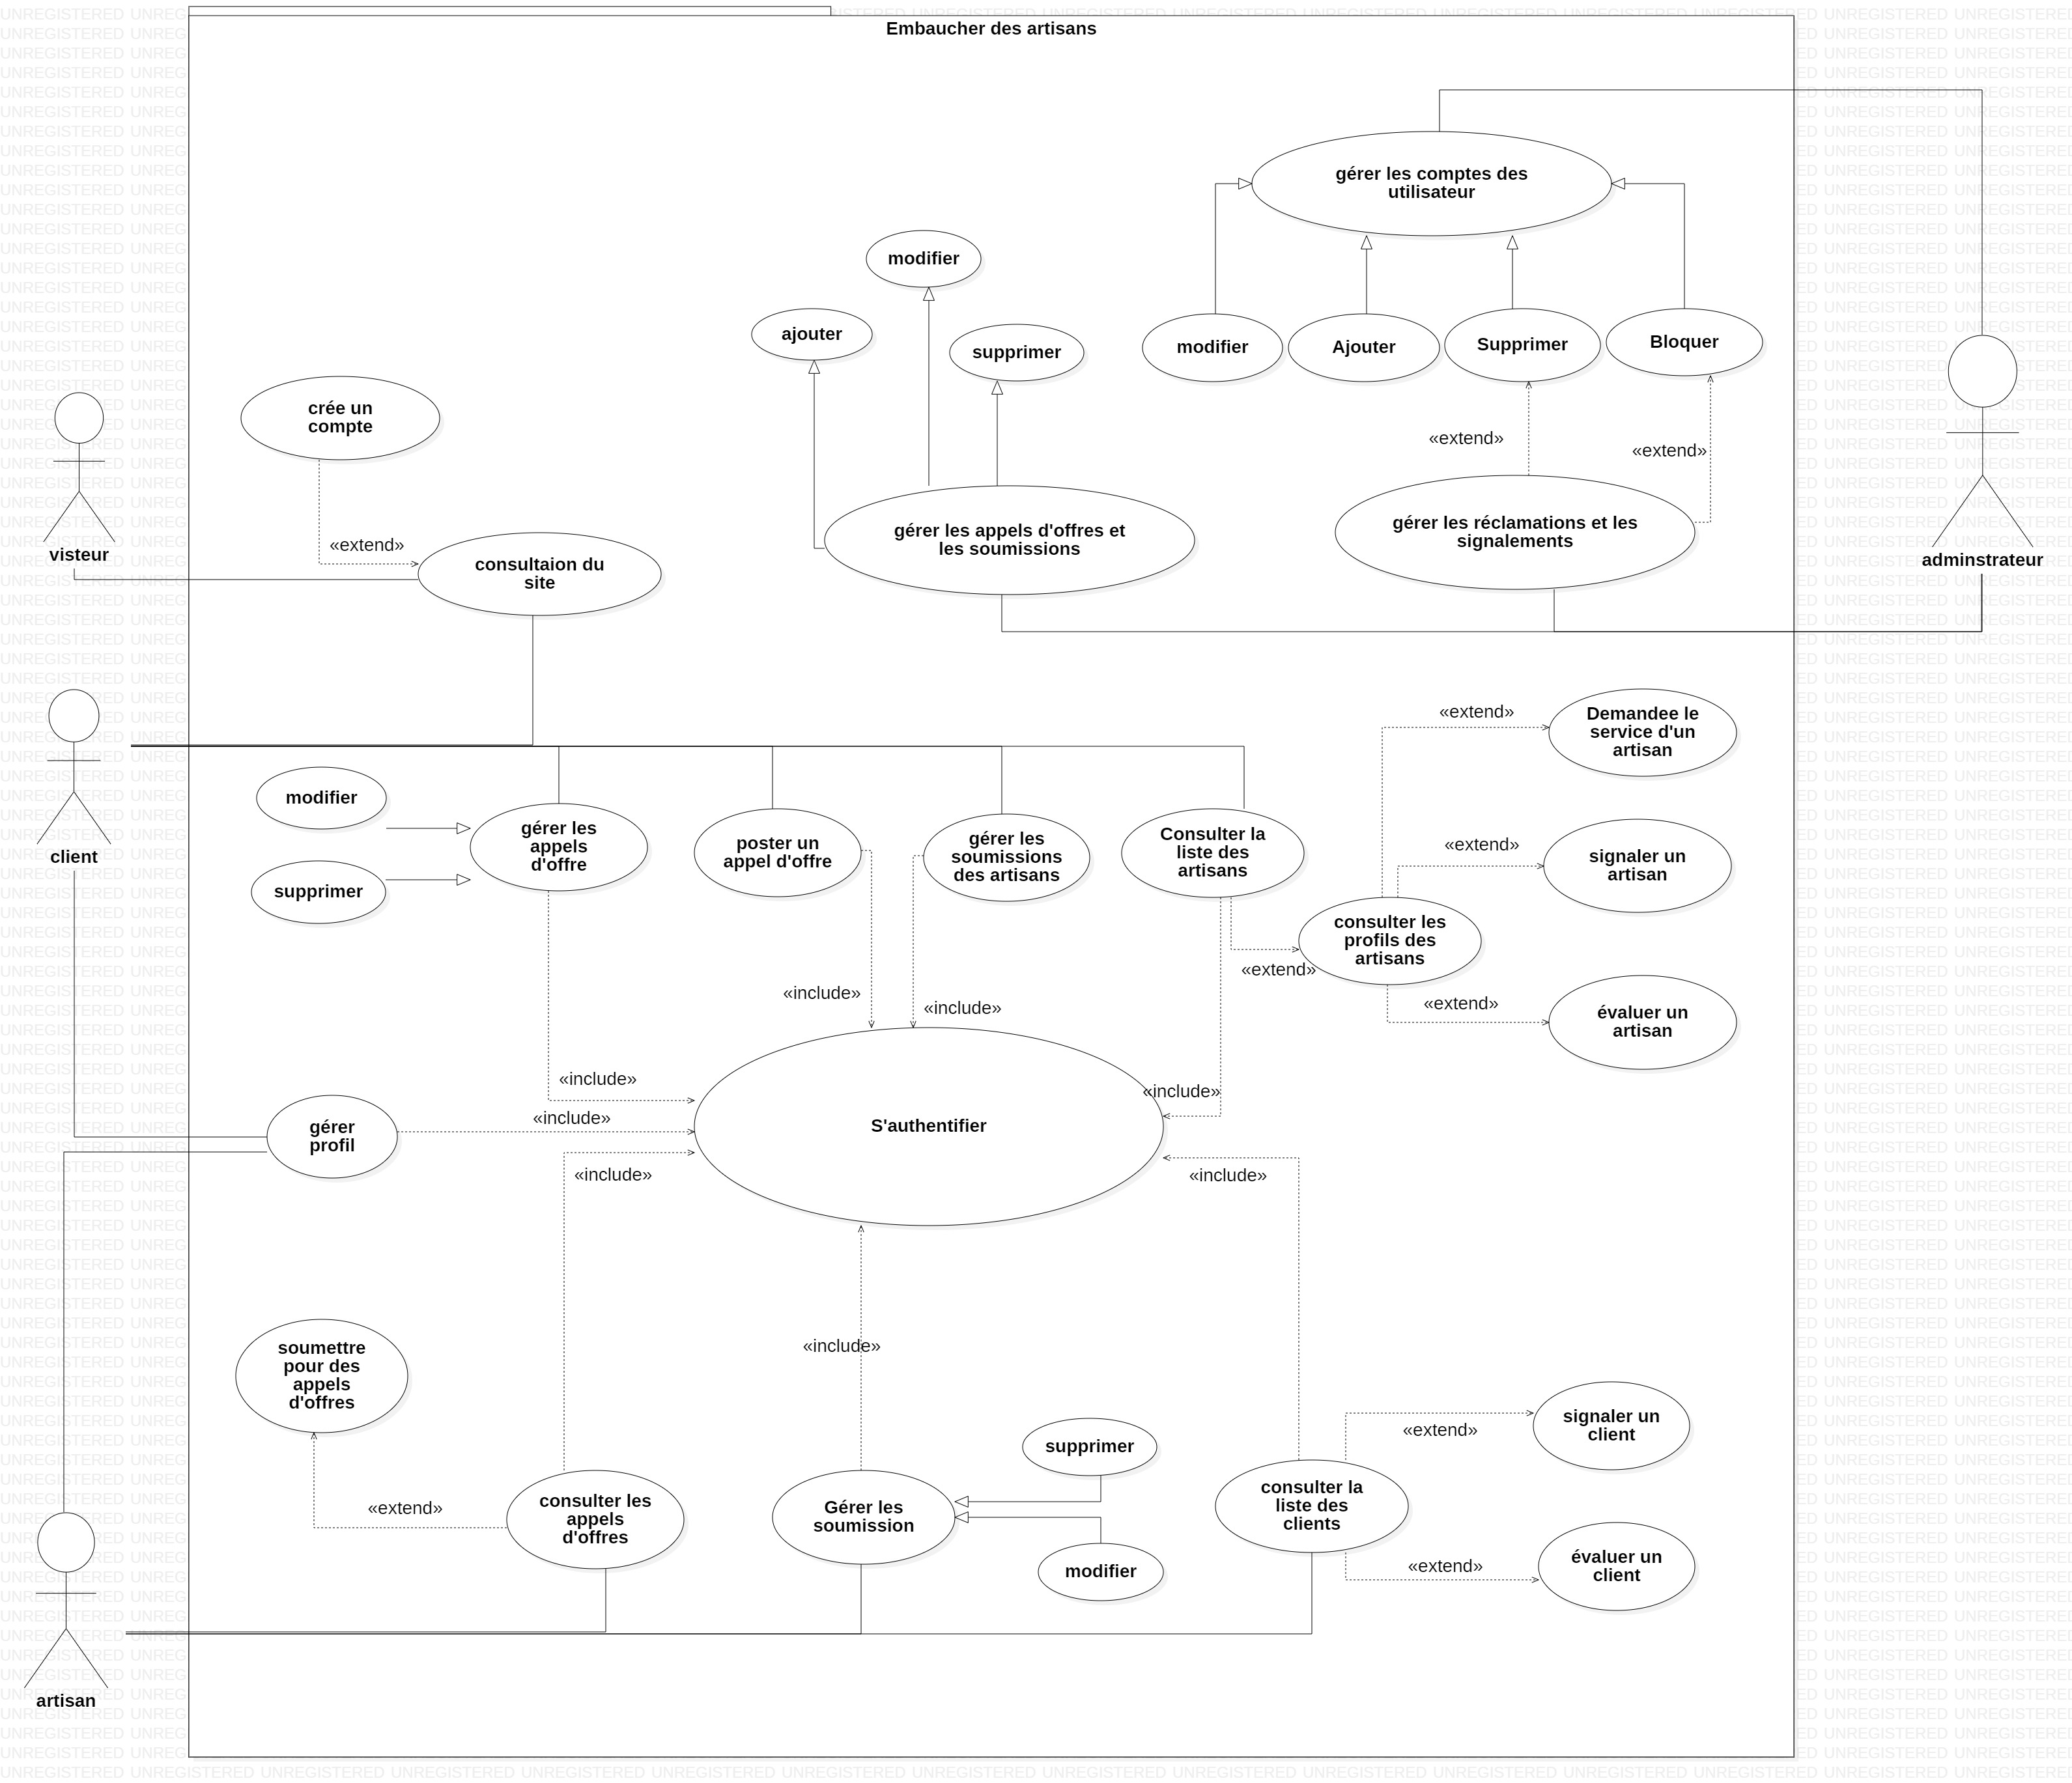
\includegraphics[scale=0.15]{UseCase.jpg}
\caption{Diagramme cas d'utilisation}
\label{fig:use case}
\end{figure}


\section{Descriptions et D.S}
Une description textuelle ou autrement dit fiche descriptive est une autre façon de communiquer les besoins du projet, elle sert à mieux clarifier le cas cité dans le diagramme cas d'utilisation.
Elle cite:\\
 - Un scénario nominal dans laquelle l'exécution se déroule comme prévu sans erreurs.\\
 - Un scénario alternatif dans laquelle l'exécution a eu un problème ou le déroulement a échoué.
 - Un scénario d'erreur ou l'exécution s'arrête complètement.
 
Un diagramme de séquence prend la description textuelle vers un niveau d'abstraction communicable et compréhensible pour mieux clarifier le cas d'utilisation avec la moindre verbosité

\pagebreak
\subsection{Cas d'utilisation Crée compte}
\renewcommand{\arraystretch}{1.3}
\begin{center}
	\begin{table}[H]
			\centering
			\tiny\begin{tabular}{ | l | m{0.51\textheight} |}
			\hline
			\rowcolor[HTML]{06a8ed}
			\textbf{Nom du cas} & Crée un compte \\
			\hline\hline
			\cellcolor[HTML]{99ccff} \textbf{Type} & Principal\\
			\hline
			\cellcolor[HTML]{99ccff} \textbf {Acteur Principal} & Visiteur\\
			\hline
			\cellcolor[HTML]{99ccff} \textbf Objective & Permet à tout visiteur du site de	crée un compte et devenir client\\
			\hline
			\cellcolor[HTML]{99ccff}\textbf {Pré-condition} & Consulter Site\\
			\hline
			\cellcolor[HTML]{99ccff} \textbf {Scénario Nominal} & \parbox{0.43\textheight}{
					\begin{enumerate}
						\vspace{0.01\textheight}
						\item Le visiteur clique << Crée Compte >>.
						\item Le site affiche le formulaire du création des comptes.
						\item Le visiteur remplis les champs affiché.
						\item Le visiteur confirme les informations.
						\item Le système vérifie informations.
						\item Le système crée un compte pour l'utilisateur et le redirige vers son profil.
						\vspace{0.01\textheight}
					\end{enumerate}}\\
			\hline
			\cellcolor[HTML]{99ccff} \textbf {Scénario Alternatif} & \parbox{0.43\textheight}{
				\begin{enumerate}
					\item \textbf{A1: Les informations du visiteur ne sont pas valides:}
						\subitem 5. Le site affiche message d'erreur.\newline						
					La séquence résume du point 2.
					
					\item \textbf{A2: Le compte existe déjà:}
						\subitem 1. Le système demande à l'utilisateur de modifier l'identifiant ou de se connecter\newline
					Le séquence reprend au point 2
				\end{enumerate}}\\
			\hline
			\cellcolor[HTML]{99ccff} \textbf{Scénario d'exception} & --- \\
			\hline
			\cellcolor[HTML]{99ccff} \textbf{Post-condition} & Un nouveau compte client sera crée\\
			\hline
		\end{tabular}
		\caption{Description Crée compte}
		\label{table:create account}
	\end{table}
	\begin{figure}[H]
		\centering
		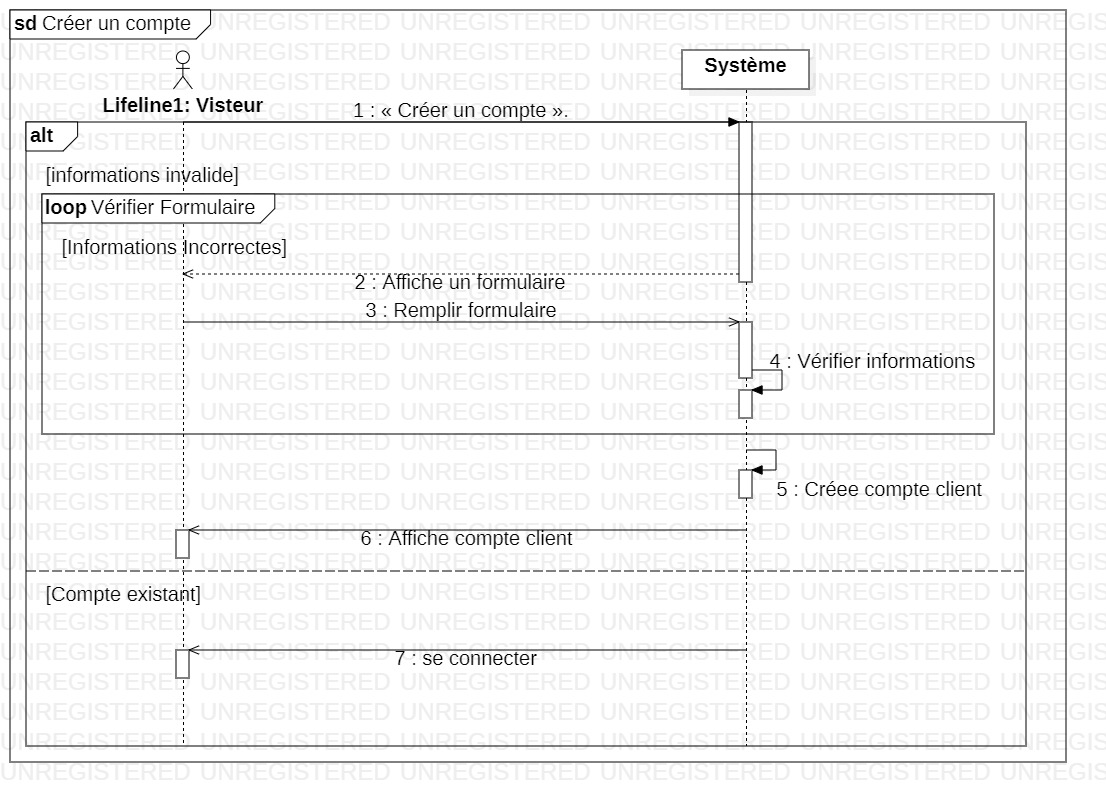
\includegraphics[scale=0.4]{CreateAccount.jpg}
		\caption{Diagramme séquence Crée un compte}
		\label{fig:seq create account}
	\end{figure}
\end{center}


\subsection{Cas d'utilisation Gérer profil (modifier)}
\renewcommand{\arraystretch}{2}
\begin{center}
	\begin{table}[H]
		\centering
		\tiny{\begin{tabular}{ | l | m{0.51\textheight} |}
			\hline
			\rowcolor[HTML]{06a8ed}
									 \textbf{Nom du cas} & Gérer profil (modifier)\\ 
			\hline \hline
			\cellcolor[HTML]{99ccff} \textbf{Type} & Principal\\
			\hline
			\cellcolor[HTML]{99ccff} \textbf{Acteur Principal} & Client, Artisans\\
			\hline
			\cellcolor[HTML]{99ccff} \textbf{Objective} & Permet à l'acteur de modifier les informations de son compte\\
			\hline
			\cellcolor[HTML]{99ccff} \textbf{Pré-condition} & S'authentifier\\
			\hline
			\cellcolor[HTML]{99ccff} \textbf{Scénario Nominal} & \parbox{0.43\textheight}{
					\begin{enumerate}
						\vspace{0.01\textheight}
						\item L'acteur clique << Gérer Profile >>.
						\item Le site affiche toutes informations cecernant l'acteur.
						\item L'acteur peut modifier les informations affichées.
						\item L'acteur confirme les modifications.
						\item Le système vérifie informations.
						\item Le système enregistre les informations.
						\item Le système affiche message de succèss.
						\vspace{0.01\textheight}
					\end{enumerate}}\\
			\hline
			\cellcolor[HTML]{99ccff} \textbf{Scénario Alternatif} & \parbox{0.43\textheight}{
				\begin{enumerate}
					\item \textbf{A1: Les informations de l'acteur ne sont pas valides:}
					\subitem 6. Le site affiche message d'erreur.\newline						
					La séquence résume du point 3.
				\end{enumerate}}\\
			\hline
			\cellcolor[HTML]{99ccff} \textbf{Scénario d'exception} & ---\\
			\hline
			\cellcolor[HTML]{99ccff} \textbf{Post-condition} & La mise-à-jour de profil de l'acteur\\
			\hline
		\end{tabular}}
		\caption{Description Modifier compte}
		\label{table:modifier account}
	\end{table}
	\begin{figure}[H]
		\centering
		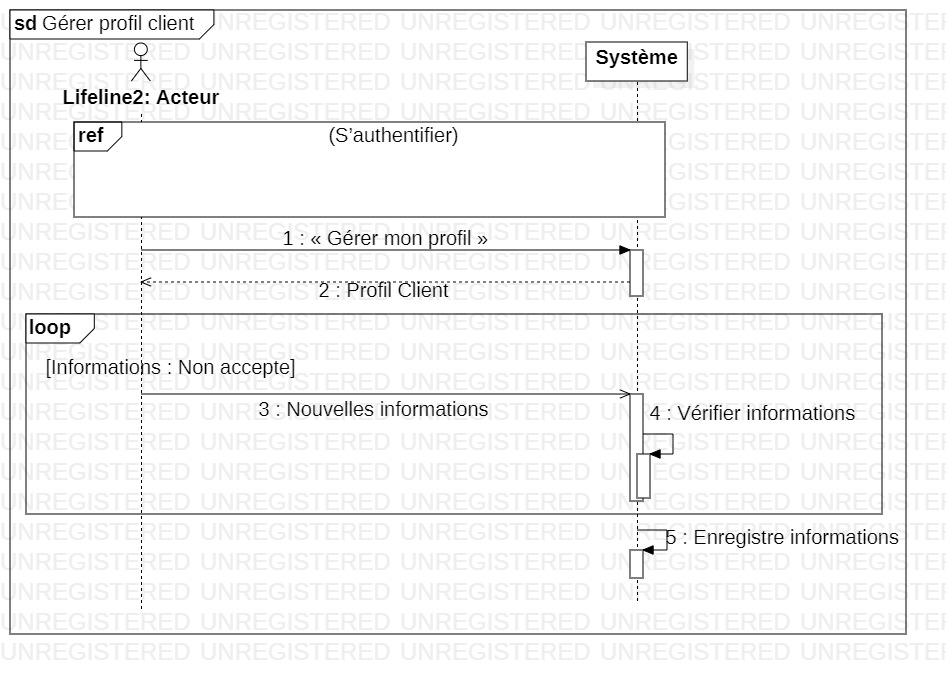
\includegraphics[scale=0.45]{ModifierProfil.jpg}
		\caption{Diagramme séquence Modifier Profil}
		\label{fig:seq update account}
	\end{figure}
\end{center}


\subsection{Cas d'utilisation Poster appel d'offre}
\renewcommand{\arraystretch}{2}
\begin{center}
	\begin{table}[H]
		\centering
		\tiny{\begin{tabular}{ | l | m{0.51\textheight}|}
				\hline
				\rowcolor[HTML]{06a8ed}
				\textbf{Nom du cas} & Poster appel d'offre \\
				\hline \hline
				\cellcolor[HTML]{99ccff} \textbf{Type} & Principal\\
				\hline
				\cellcolor[HTML]{99ccff} \textbf{Acteur Principal} & Client\\
				\hline
				\cellcolor[HTML]{99ccff} \textbf{Objective} & Permet au client de poster un offre de travail pour les artisans\\
				\hline
				\cellcolor[HTML]{99ccff} \textbf{Pré-condition} & S'authentifier\\
				\hline
				\cellcolor[HTML]{99ccff} \textbf{Scénario Nominal} & \parbox{0.43\textheight}{
					\begin{enumerate}
						\vspace{0.01\textheight}
						\item L'acteur clique << Poster appel d'offre >>.
						\item Le site affiche un formualire a remplir.
						\item L'acteur remplis les champs.
						\item L'acteur confirme l'appel.
						\item Le système vérifie informations.
						\item Le système crée un appel d'offre.
						\vspace{0.01\textheight}
				\end{enumerate}}\\
				\hline
				\cellcolor[HTML]{99ccff} \textbf{Scénario Alternatif} & \parbox{0.43\textheight}{
					\begin{enumerate}
						\item \textbf{A1: Les informations du client ne sont pas valides:}
							\subitem 6. Le site affiche message d'erreur.\newline						
						La séquence résume du point 3.
						\item \textbf{A2: Le client annule / ne confirme pas l'appel:}
							\subitem 5. Le site retourne a la page d'acceuile
				\end{enumerate}}\\
				\hline
				\cellcolor[HTML]{99ccff} \textbf{Scénario d'exception} & ---\\
				\hline
				\cellcolor[HTML]{99ccff} \textbf{Post-condition} & Un nouveau appel d'offre sera crée\\
				\hline
		\end{tabular}}
		\caption{Description Poster un appel d'offre}
		\label{table:post appel offre}
	\end{table}
	\begin{figure}[H]
		\centering
		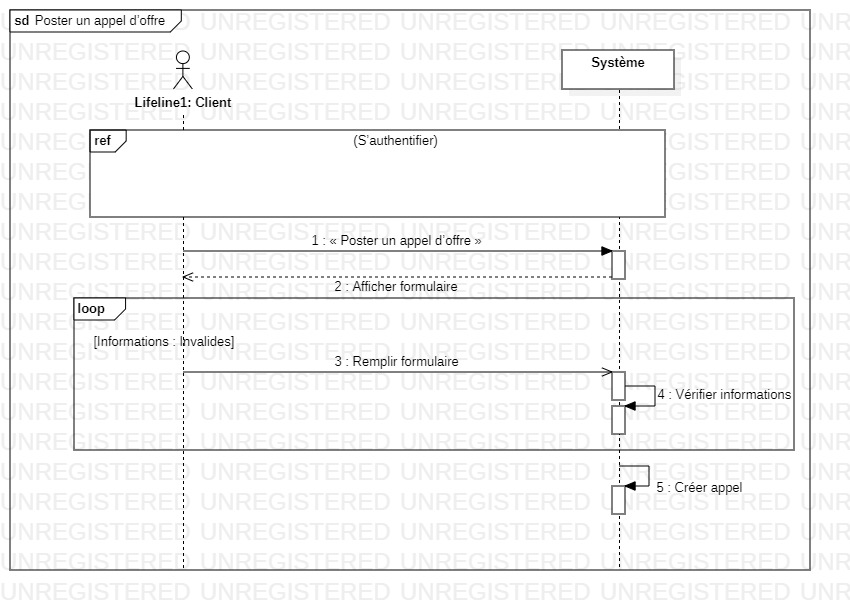
\includegraphics[scale=0.45]{PosterAppelOffre.jpg}
		\caption{Diagramme séquence Poster Appel Offre}
		\label{fig:seq post appel offre}
	\end{figure}
\end{center}


\subsection{Cas d'utilisation Soumission appel d'offre}
\renewcommand{\arraystretch}{2}
\begin{center}
	\begin{table}[H]
		\centering
		\tiny{\begin{tabular}{ | l | m{0.51\textheight}|}
				\hline
				\rowcolor[HTML]{06a8ed}
				\textbf{Nom du cas} & Soumission appel d'offre \\
				\hline\hline
				\cellcolor[HTML]{99ccff} \textbf{Type} & Principal \\
				\hline
				\cellcolor[HTML]{99ccff} \textbf{Acteur Principal} & Artisan\\
				\hline
				\cellcolor[HTML]{99ccff} \textbf{Objective} & Permet à artisan de soumettre un appel d'offre à un client\\
				\hline
				\cellcolor[HTML]{99ccff} \textbf{Pré-condition} & S'authentifier\\
				\hline
				\cellcolor[HTML]{99ccff} \textbf{Scénario Nominal} & \parbox{0.43\textheight}{
					\begin{enumerate}
						\vspace{0.01\textheight}
						\item Artisan cliquer sur << Soumettre appel d’offre >>
						\item Le système affiche la liste des offres
						\item L'artisan soumis un ou plusieurs offres
						\item Le système sauvegarde la soumission
						\item Le système notifie le client
						\vspace{0.01\textheight}
				\end{enumerate}}\\
				\hline
				\cellcolor[HTML]{99ccff} \textbf{Scénario Alternatif} & --- \\
				\hline
				\cellcolor[HTML]{99ccff} \textbf{Scénario d'exception} & --- \\
				\hline
				\cellcolor[HTML]{99ccff} \textbf{Post-condition} & Un appel d'offre sera soumis\\
				\hline
		\end{tabular}}
		\caption{Description Soumission d'un appel d'offre}
		\label{table:soumettre offre}
	\end{table}
	\begin{figure}[H]
		\centering
		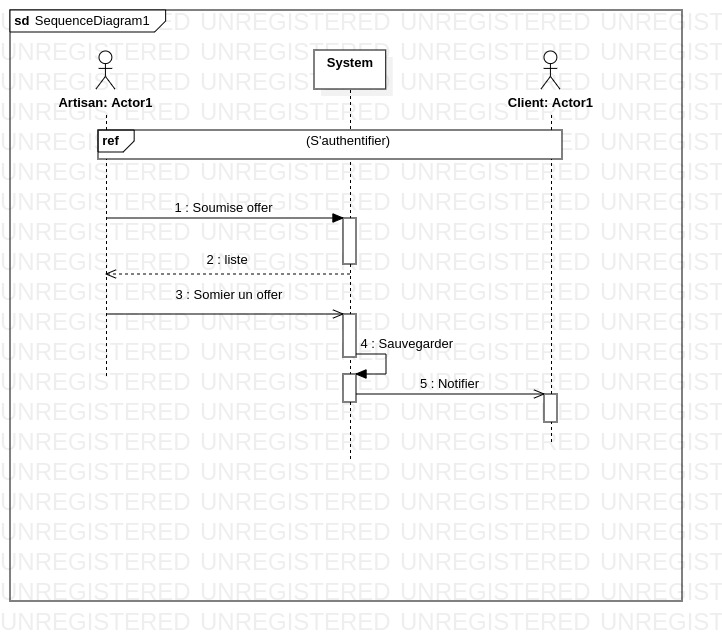
\includegraphics[scale=0.45]{SoumttreOffre.jpg}
		\caption{Diagramme séquence Soumettre un appel d'offre}
		\label{fig:seq soumettre offre}
	\end{figure}
\end{center}


\subsection{Cas d'utilisation Signaler un utilisateur}
\renewcommand{\arraystretch}{2}
\begin{center}
	\begin{table}[H]
		\centering
		\tiny{\begin{tabular}{ | l | m{0.51\textheight}|}
				\hline
				\rowcolor[HTML]{06a8ed}
				\textbf{Nom du cas} & Signaler un utilisateur \\
				\hline\hline
				\cellcolor[HTML]{99ccff} \textbf{Type} & Principal \\
				\hline
				\cellcolor[HTML]{99ccff} \textbf{Acteur Principal} & Client, Artisan\\
				\hline
				\cellcolor[HTML]{99ccff} \textbf{Objective} & Permet à un utilisateur de signaler un autre utilisateur\\
				\hline
				\cellcolor[HTML]{99ccff} \textbf{Pré-condition} & Consulter Profil\\
				\hline
				\cellcolor[HTML]{99ccff} \textbf{Scénario Nominal} & \parbox{0.43\textheight}{
					\begin{enumerate}
						\vspace{0.01\textheight}
						\item L'acteur clique consulte le profil de l'utilisateur.
						\item Le site affiche le profil de l'utilisateur.
						\item L'acteur clique sur << Signaler >>.
						\item Le système affiche un forumalire a remplir.
						\item L'acteur remplis le formulaire.
						\item Le système vérifie informations.
						\item Le système envoie sauvgarde le rapport et l'envoie aux administrateurs.
						\vspace{0.01\textheight}
				\end{enumerate}}\\
				\hline
				\cellcolor[HTML]{99ccff} \textbf{Scénario Alternatif} & \parbox{0.43\textheight}{
					\begin{enumerate}
						\item \textbf{A1: Les informations du formulaire ne sont pas valides:}
						\subitem 7. Le site affiche message d'erreur.\newline						
						La séquence résume du point 4.
						\item \textbf{A2: Le client annule / ne confirme pas l'appel:}
						\subitem 5. Le site retourne a la page d'acceuile
				\end{enumerate}}\\
				\hline
				\cellcolor[HTML]{99ccff} \textbf{Scénario d'exception} & --- \\
				\hline
				\cellcolor[HTML]{99ccff} \textbf{Post-condition} & Un rapport sera envoyé aux administrateurs\\
				\hline
		\end{tabular}}
		\caption{Description Signaler un utilisateur}
		\label{table:signaler utilisateur}
	\end{table}
	\begin{figure}[H]
		\centering
		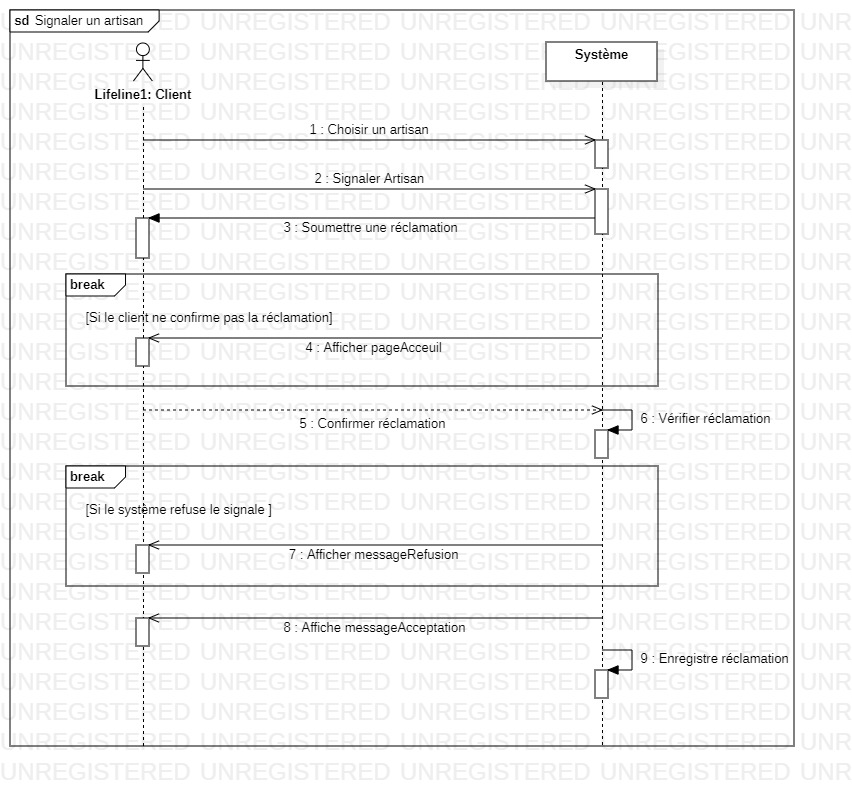
\includegraphics[scale=0.44]{SignalerUtilisateur.jpg}
		\caption{Diagramme séquence Signaler un Utilisateur}
		\label{fig:seq signaler utilisateur}
	\end{figure}
\end{center}


\subsection{Cas d'utilisation Bloquer un utilisateur}
\renewcommand{\arraystretch}{2}
\begin{center}
	\begin{table}[H]
		\centering
		\tiny{\begin{tabular}{ | l | m{0.51\textheight}|}
				\hline
				\rowcolor[HTML]{06a8ed}
				\textbf{Nom du cas} & Bloquer un utilisateur \\
				\hline\hline
				\cellcolor[HTML]{99ccff} \textbf{Type} & Principal \\
				\hline
				\cellcolor[HTML]{99ccff} \textbf{Acteur Principal} & Administrateur\\
				\hline
				\cellcolor[HTML]{99ccff} \textbf{Objective} & Permet à un administrateur de bloquer (banner) un utilisateur\\
				\hline
				\cellcolor[HTML]{99ccff} \textbf{Pré-condition} & S'authentifier\\
				\hline
				\cellcolor[HTML]{99ccff} \textbf{Scénario Nominal} & \parbox{0.43\textheight}{
					\begin{enumerate}
						\vspace{0.01\textheight}
						    \item L’acteur visite la fenêtre d’édition
							\item Une liste de tous les utilisateurs sera affichée
							\item L’administrateur clique sur l’utilisateur voulu
							\item L’admin clique sur bouton bloquer
							\item Un message confirmation s’affichera
							\item L’admin confirme son action
							\item Le systeme banne l'utilisateur
						\vspace{0.01\textheight}
				\end{enumerate}}\\
				\hline
				\cellcolor[HTML]{99ccff} \textbf{Scénario Alternatif} & \parbox{0.43\textheight}{
					\begin{enumerate}
						\item \textbf{A1: L'administrateur annule l'action:}
						\subitem 7. Le systeme affiche la page d'acceuille.\newline						
						\item \textbf{A2: L'utilisateur est un autre administrateur:}
						\subitem 7. Le systeme affiche un message d'erreur.
						\subitem 8. Le systeme affiche la page d'acceuille.
				\end{enumerate}}\\
				\hline
				\cellcolor[HTML]{99ccff} \textbf{Scénario d'exception} & --- \\
				\hline
				\cellcolor[HTML]{99ccff} \textbf{Post-condition} & L'utilisateur sera banné\\
				\hline
		\end{tabular}}
		\caption{Description Bloquer un utilisateur}
		\label{table:bloquer utilisateur}
	\end{table}
	\begin{figure}[H]
		\centering
		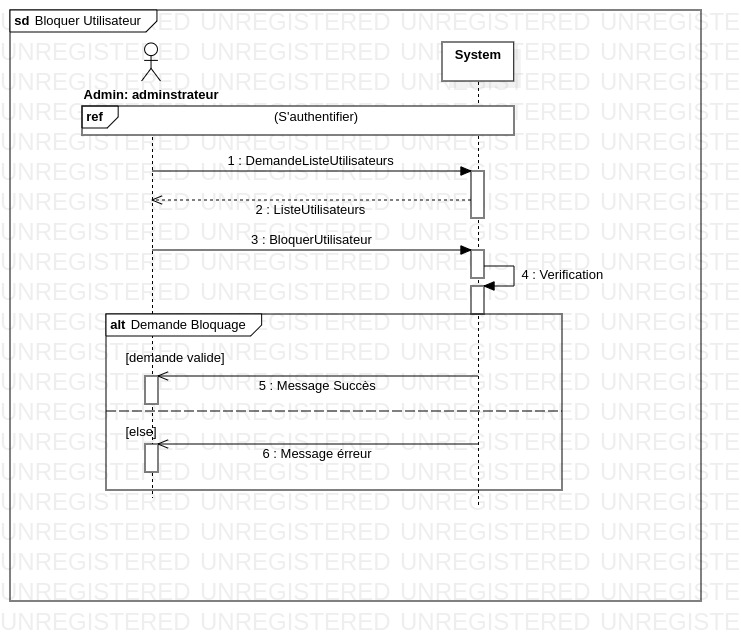
\includegraphics[scale=0.52]{BloquerUtilisateur.jpg}
		\caption{Diagramme séquence Bloquer un Utilisateur}
		\label{fig:seq bloquer utilisateur}
	\end{figure}
\end{center}


\subsection{Cas d'utilisation Gérer réclamations et signalements}
\renewcommand{\arraystretch}{2}
\begin{center}
	\begin{table}[H]
		\centering
		\tiny{\begin{tabular}{ | l | m{0.51\textheight}|}
				\hline
				\rowcolor[HTML]{06a8ed}
				\textbf{Nom du cas} & Gérer réclamations et signalements \\
				\hline\hline
				\cellcolor[HTML]{99ccff} \textbf{Type} & Principal \\
				\hline
				\cellcolor[HTML]{99ccff} \textbf{Acteur Principal} & Administrateur\\
				\hline
				\cellcolor[HTML]{99ccff} \textbf{Objective} & Permet à un administrateur de Gérer une réclamations et de prendre une action\\
				\hline
				\cellcolor[HTML]{99ccff} \textbf{Pré-condition} & S'authentifier\\
				\hline
				\cellcolor[HTML]{99ccff} \textbf{Scénario Nominal} & \parbox{0.43\textheight}{
					\begin{enumerate}
						\vspace{0.01\textheight}
						\item L’acteur visite la fenêtre des réclamations et signalements
						\item Une liste de tous les réclamations et signalements s’affiche
						\item L’administrateur clique sur une réclamation / signalement
						\item Détailles de la réclamation / signalement s’affiche
						\item L’administrateur, après avoir lu la réclamation, peut soit, en cliquant sur un bouton, l’accepter, la refuser ou contacter la source du réclamation pour plus de détails
						\item En cas d’accepter la réclamation, l’admin sera redirigé vers une nouvelle page (gérer compte utilisateur) pour choisir une action  
						\vspace{0.01\textheight}
				\end{enumerate}}\\
				\hline
				\cellcolor[HTML]{99ccff} \textbf{Scénario Alternatif} & --- \\
				\hline
				\cellcolor[HTML]{99ccff} \textbf{Scénario d'exception} & --- \\
				\hline
				\cellcolor[HTML]{99ccff} \textbf{Post-condition} & La réclamation sera résolu\\
				\hline
		\end{tabular}}
		\caption{Description Gérer réclamations et signalements}
		\label{table:gerer reclamation}
	\end{table}
	\begin{figure}[H]
		\centering
		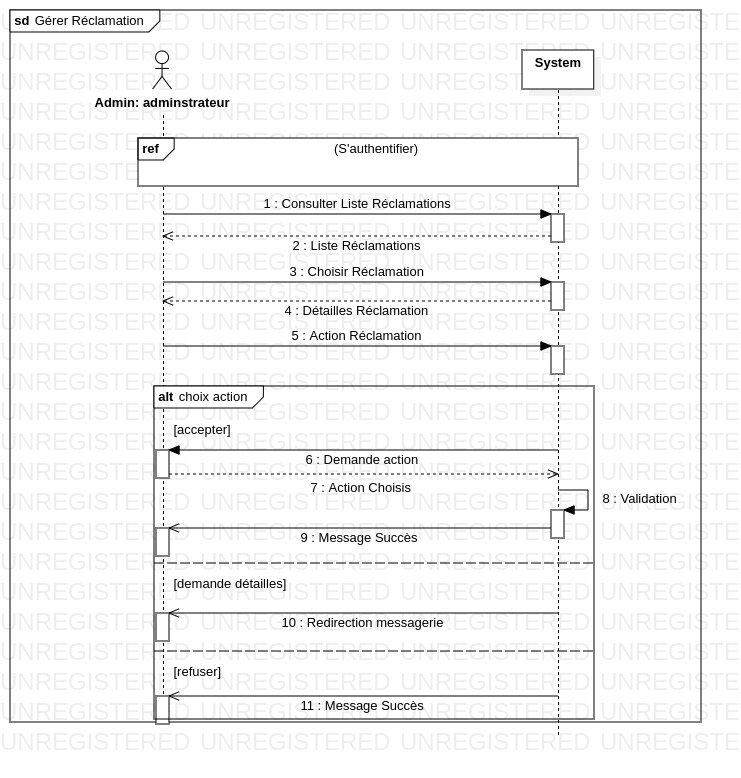
\includegraphics[scale=0.45]{GererReclamation.jpg}
		\caption{Diagramme séquence Gérer réclamations et signalements}
		\label{fig:seq gere reclamation}
	\end{figure}
\end{center}

\section{Conclusion}
Dans ce chapitre, nous avons présenté l’analyse des besoins dont on identifient les acteurs / utilisateurs qui interagissent avec notre future application suivi par la spécification des besoins fonctionnels et techniques(non-fonctionnels), modélisés sous forme des diagrammes.\\

On finalise par la description détaillée et les diagrammes de séquences des cas dont on a jugé important ou intéressant.

\vspace{0.01\textheight}
On se basant sur les descriptions et diagrammes précédents, on entame le deuxième chapitre du conception

\chapter{Conception}


\section{Introduction}
Les activités d'expression des besoins et d'analyse ont permis de définir quel système a construire.

L’activité de conception s’intéresse à la façon de construire le système, elle propose donc une solution qui doit satisfaire aux besoins du système, une décomposition modulaire y est souvent recommandée.

L’architecture du logiciel ainsi que chacun de ses constituants: informations traitées, traitements effectués, résultats fournis, contraintes à respecter.La conception orientée objet (COO) consiste à concevoir l’organisation des modules (classes) du logiciel et du stockage des données persistantes.

\begin{itemize}
	\item La conception constitue un point de départ à l’implémentation 
	\item décompose le travail d’implémentation en sous-systèmes.
	\item crée une abstraction transparente de l’implémentation. 
\end{itemize}

\section{Modèle du domaine}
Le diagramme de classes en montre la structure interne. Il permet de fournir une représentation abstraite des objets du système qui vont interagir ensemble pour réaliser les cas d’utilisation. Il est important de noter qu’un même objet peut très bien intervenir dans la réalisation de plusieurs cas d’utilisation.

\begin{figure}[H]
	\centering
	
\includegraphics[scale=0.5]{DiagrammeDeClasse.png}
	\caption{Diagramme de classe}
	\label{fig:diagramme class}
\end{figure}

\section{Diagrammes d’activité}
Les diagrammes d’activités sont également utiles dans la phase de réalisation car ils permettent une description si précise des traitements qu’elle autorise la génération automatique du code.

\subsection{Modifier Profil}

\begin{figure}[H]
	\centering
	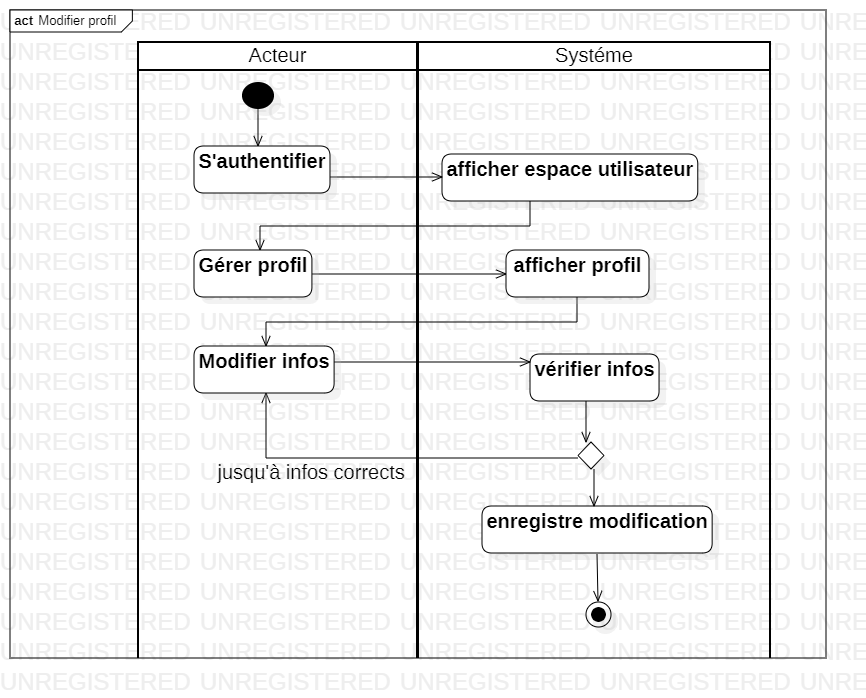
\includegraphics[scale=0.5]{CliModifierProfil.png}
	\caption{Diagramme d'action Modifier Profil}
	\label{fig:action modifier profil}
\end{figure}

\subsection{Poster Un appel d'offre}

\begin{figure}[H]
	\centering
	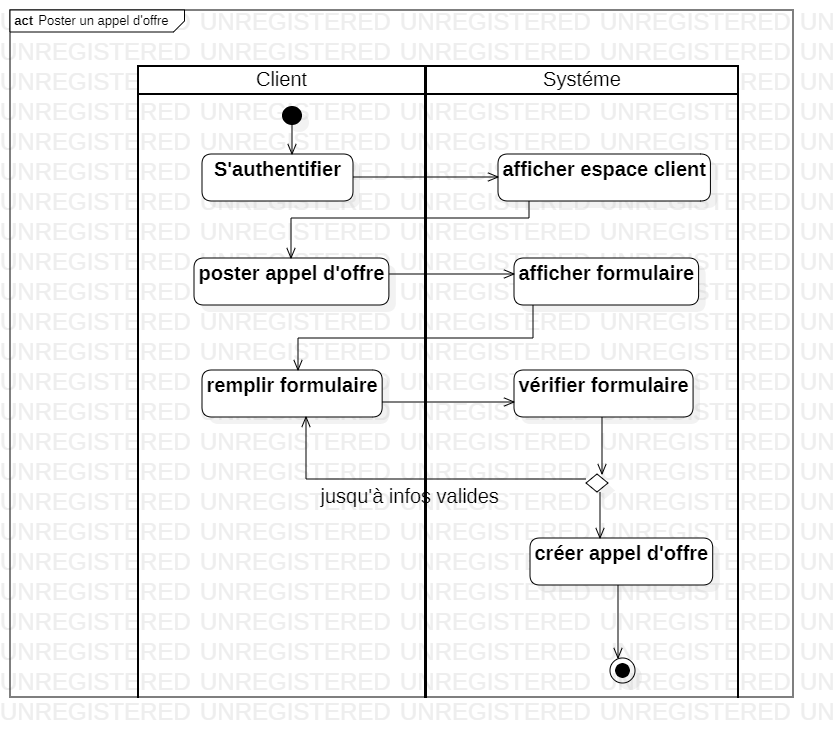
\includegraphics[scale=0.5]{CliPosterAppel.png}
	\caption{Diagramme d'action Poster Appel}
	\label{fig:action poster appel}
\end{figure}

\subsection{Signaler}

\begin{figure}[H]
	\centering
	
\includegraphics[scale=0.5]{signaler.png}
	\caption{Diagramme d'action signaler}
	\label{fig:action signaler}
\end{figure}

\subsection{Soumettre appel d’offre}

\begin{figure}[H]
	\centering
	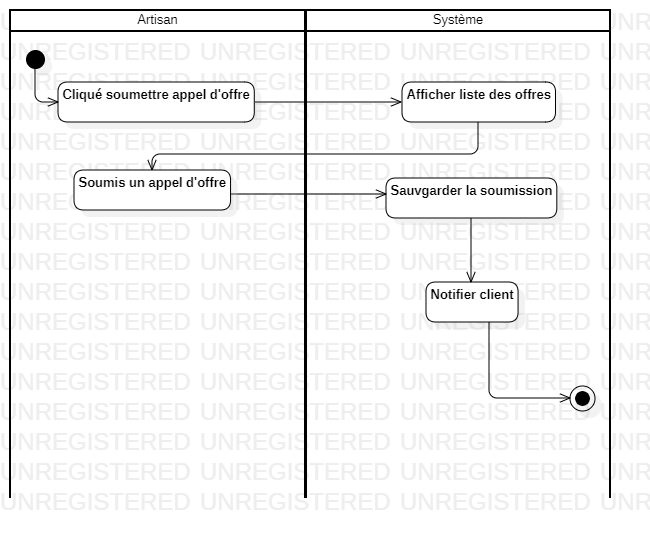
\includegraphics[scale=0.5]{Soumettre appel d'offre.png}
	\caption{Diagramme d'action Soumettre appel d'offre}
	\label{fig:action soumettre appel d'offre}
\end{figure}

\subsection{Bloquer Utilisateur}

\begin{figure}[H]
	\centering
	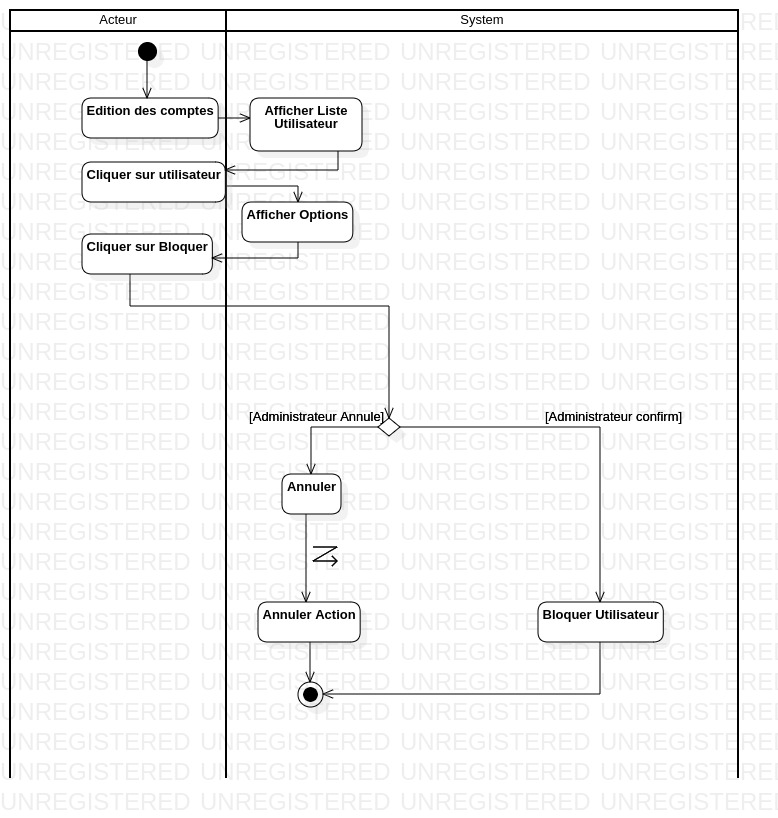
\includegraphics[scale=0.5]{BloquerUtilisateurAction.jpg}
	\caption{Diagramme d'action Bloquer utilisateur}
	\label{fig:action bloquer user}
\end{figure}

\subsection{Gérer Réclamation}

\begin{figure}[H]
	\centering
	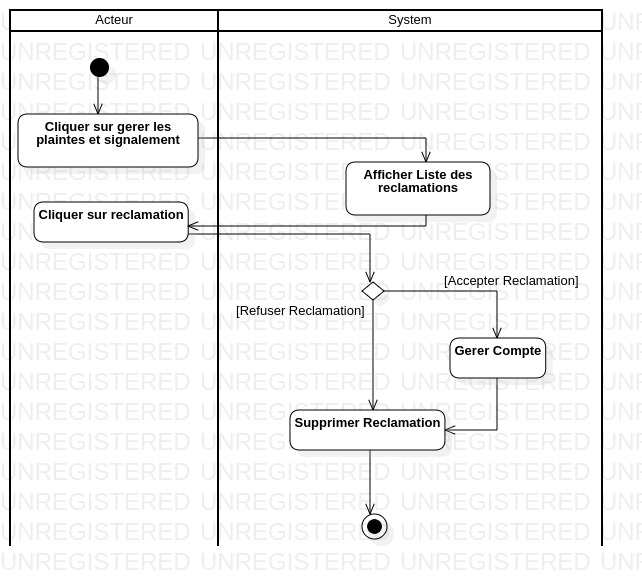
\includegraphics[scale=0.5]{GereReclamationAction.jpg}
	\caption{Diagramme d'action Gérer réclamations}
	\label{fig:action gerer reclamation}
\end{figure}

\section{Schéma de base de données}
\subsection{Règles de passages}
\begin{enumerate}
	\item Transformation des classes: Les classes dans un diagramme de classes sont transformées aux des relations dans  modèle relationnelle dans la base de données et des tables dans le modèle physique .
	
	\item Transformation des attributs : Les attributs des classes dans un diagramme de classes sont considérés comme des attributs pour les relations dans le modèle relationnel dans la base de données et des colonnes dans les tables dans le modèle physique .
	L’identifiant de classe est transformé en une clé primaire dans la BD .
	
	\item Transformation des associations : 
		\subitem Association de 1 à N : Pour chaque classe A de diagramme , elle a une association de 1 à N avec classe B , il faut ajouter l’identifiant de la classe B - clé primaire dans BD - comme un clé étrangère dans BD .
		
		\subitem Association de 1: Il existe deux solutions :
		\begin{itemize}
			\item Si les deux multiplicités minimales sont à un, il est préférable de fusionner les deux classes en une seule .
			\item Sinon on fait la même chose pour une association de 1 à N .
		\end{itemize}
	
		\subitem Association de 0 à N: Chaque classe-association est représentée par une relation. La clé primaire de cette relation est la concaténation des identifiants - clés primaires-  des classes connectées à l'association
		
	\item Transformation des compositions: Chaque élément de la classe composite est représenté par une relation , il faut ajouter l’identifiant - clé primaire -   de cette classe comme un clé étrangère à l'élément de la composite.
	
	\item Transformation d'héritage: Chaque classe mère ou fille est représentée par une relation . L’identifiant - clé primaire - de la classe mère est ajouté comme un clé primaire et clé étrangère à la fois dans la classe fille.
	
\end{enumerate}

\subsection{Les relations de la base de données}

\noindent Utilisateur ( \underline{idUtilisateur} , nome , prénom , email , motPasse , téléphone , sexe , dateNaissance , adresse )\\
Admin ( \underline{idAdmin} , \#idUtilisateur )\\
Client ( \underline{idClient} , \#idUtilisateur )\\
Signale ( \underline{idSignale} , date , \#idClient , \#idArtisan )\\
Réclamation ( \underline{idReclamation} , description , \#idSignale , \#idClient , \#idAdmin , \#idArtisan )\\
Evaluation ( \underline{idEvaluation} , nmrEvaluation , \#idClient ,\#idArtisan )\\
Soumissions ( \underline{idSoumissions} , description , \#idAppel , \#idArtisan )\\
Appel d’offre ( \underline{idAppel} , dateDébut , dateFin , catégorie ,  prix , adresse ,\#idClient , \#idArtisan , \#idAdmin )\\

\begin{figure}[H]
	\centering
	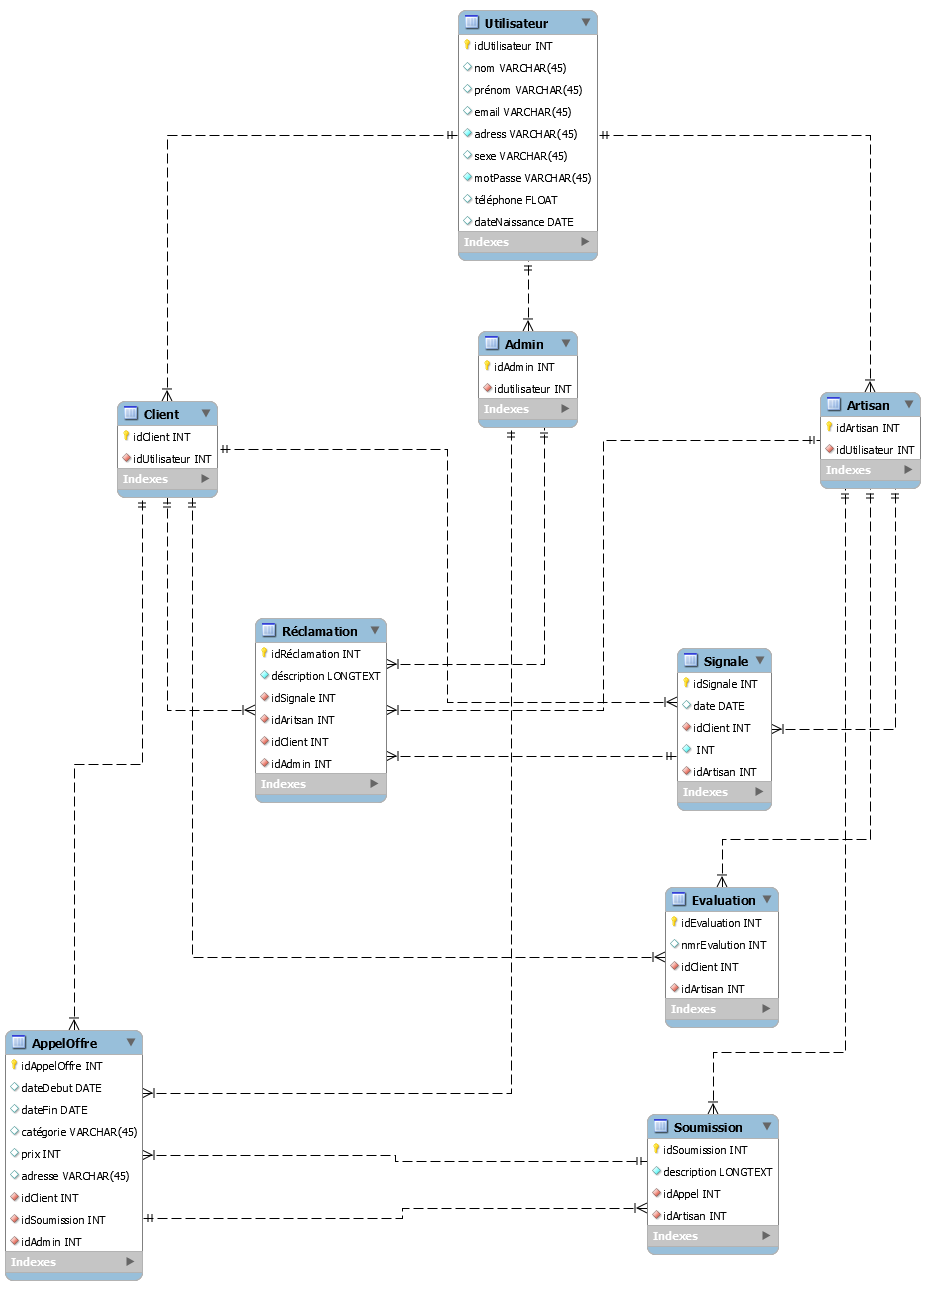
\includegraphics[scale=0.5]{SchemaDB.png}
	\caption{Schéma Base de donnée}
	\label{figure: scheme bd}
\end{figure}

\section{Conclusion}
Durant ce chapitre nous avons , nous avons détailler notre projet, nous avons réalisé une analyse profonde de la solution adaptée en précisant les différentes fonctionnalités du système 


\end{document}
